\documentclass[12pt,a4paper]{article}

\usepackage[dutch]{babel}
\usepackage{listings}

\usepackage[]{algorithm2e}

% Voor todo's
\usepackage{todonotes}

% Voor wiskunde
\usepackage{amsmath}
\usepackage{amsfonts}
\usepackage{amssymb}

% Om het totaal aantal pagina's te tellen
\usepackage{lastpage}

% Voor tekeningen
\usepackage{tikz}
\usetikzlibrary{decorations}
\usetikzlibrary{calc}

% Nog tekeningen
\usepackage{pgfplots}

% Om de marges aan te passen
\usepackage[left=2cm,right=2cm,top=2cm,bottom=2cm]{geometry}

% Voor headers en footers
\usepackage{fancyhdr}
\pagestyle{fancy}

\lhead{Tom Sydney Kerckhove \& Xavier Go\'as Aguililla}
\rhead{\thepage /\pageref{LastPage}}

\lfoot{Practicum}
\cfoot{Toepassingen van Meetkunde in Informatica}
\rfoot{Snijdende Cirkels}

\renewcommand{\headrulewidth}{0.4pt}
\renewcommand{\footrulewidth}{0.4pt}

\begin{document}
\begin{titlepage}

\newcommand{\HRule}{\rule{\linewidth}{0.5mm}}
\center
\textsc{\LARGE KU Leuven}\\[1.5cm]
\textsc{\Large Practicum:}\\[0.5cm]
\textsc{\large Snijdende Cirkels}\\[0.5cm]

\HRule \\[0.4cm]
{ \huge \bfseries Verslag}\\[0.4cm]
\HRule \\[1.5cm]

\begin{minipage}{0.4\textwidth}
\begin{flushleft} \large
\emph{Authors:}\\
Tom Sydney \textsc{Kerckhove}\\
Xavier \textsc{Go\'as Aguililla}
\end{flushleft}
\end{minipage}
~
\begin{minipage}{0.4\textwidth}
\begin{flushright} \large
\emph{Supervisor:} \\
Prof. D. \textsc{Roose}
\end{flushright}
\end{minipage}\\[4cm]

{\large 15 mei 2014}\\[3cm]
\vfill

\end{titlepage}

\tableofcontents
\section{Inleiding}
%% \todo{inleiding}


\section{Algoritmen}

\subsection{Snijpunt van twee cirkels berekenen}
\label{sec:snijpunt}

\begin{algorithm}[H]
  \KwData{twee cirkels, C en C' met resp middelpunten $p_{1}, p_{2}$ en stralen $r_{1}, r_{2}$}
  \KwResult{waar als en slechts als de twee cirkels snijden}
  d $\leftarrow$ afstand(p1,p2)\\
  \eIf{($d \leq r_1 + r_2) \land (d \geq abs (r_1 - r_2))$}{
    \Return{true}
  }{
    \Return{false}
  }

 \caption{Nagaan of twee cirkels snijden}
\end{algorithm}

\begin{algorithm}[H]
  \KwData{twee cirkels, C en C' met resp. middelpunten $p_{1} = (x_1,y_1), p_{2} = (x_2,y_2)$ en stralen $r_{1}, r_{2}$}
  \KwResult{geen, of twee snijpunten van de twee cirkels (die dan identiek zijn)}
  \eIf{$circlesIntersect(c1, c2) \land c1 \neq c2$}{
    $d \leftarrow afstand(p1, p2)$\\
    $d' \leftarrow d*d$\\
    $\alpha \leftarrow (r1*r1-r2*r2)/(2*d')$\\
    $s \leftarrow ((x1+x2)/2) + (x2-x1) * \alpha$\\
    $t \leftarrow ((y1+y2)/2) + (y2-y1) * \alpha$\\
    $\delta \leftarrow (1/4) * sqrt ( (d+r1+r2)*(d+r1-r2)*(d-r1+r2)*(r1+r2-d)  )$\\
    $x_1' \leftarrow s + 2*(y1-y2)/d'*\delta$\\
    $x_2' \leftarrow s - 2*(y1-y2)/d'*\delta$\\
    $y_1' \leftarrow t - 2*(x1-x2)/d'*\delta$\\
    $y_2' \leftarrow t + 2*(x1-x2)/d'*\delta$\\
    \Return{$\left\{(x_1,y_1),(x_2,y_2)\right\}$}
  }{
    \Return{$\varnothing$}
  }

 \caption{Snijpunten van twee cirkels berekenen}
\end{algorithm}

\subsection{Na\"ief}
\label{sec:naief}

De naïeve aanpak is gegarandeerd $O(n^2)$ en kunnen we als volgt beschrijven:

\begin{algorithm}[H]
  \KwData{een lijst van $n$ cirkels C, gegeven door hun middelpunt en straal}
  \KwResult{een verzameling van $S$ snijpunten R van de cirkels in C}
  S = $\varnothing$\;
  \For{$i\leftarrow 1$ \KwTo $n$}{
    \For{$j\leftarrow i$ \KwTo $n$}{
      $S = S \cup circleIntersection(c(i),c(j))$
    }

  }
 \caption{Na\"ieve aanpak (imperatief)}
\end{algorithm}

\subsection{Kwadratisch}
\label{sec:kwadratisch}

\subsection{Linearitmisch}
\label{sec:linearitmisch}


\section{Experimenten}
%% \todo{Doubling ratio experiment voor runtime}
%% \todo{experiment ivm stralen}

\begin{figure}[H]
  \centering
  % \resizebox {\textwidth} {!} {
    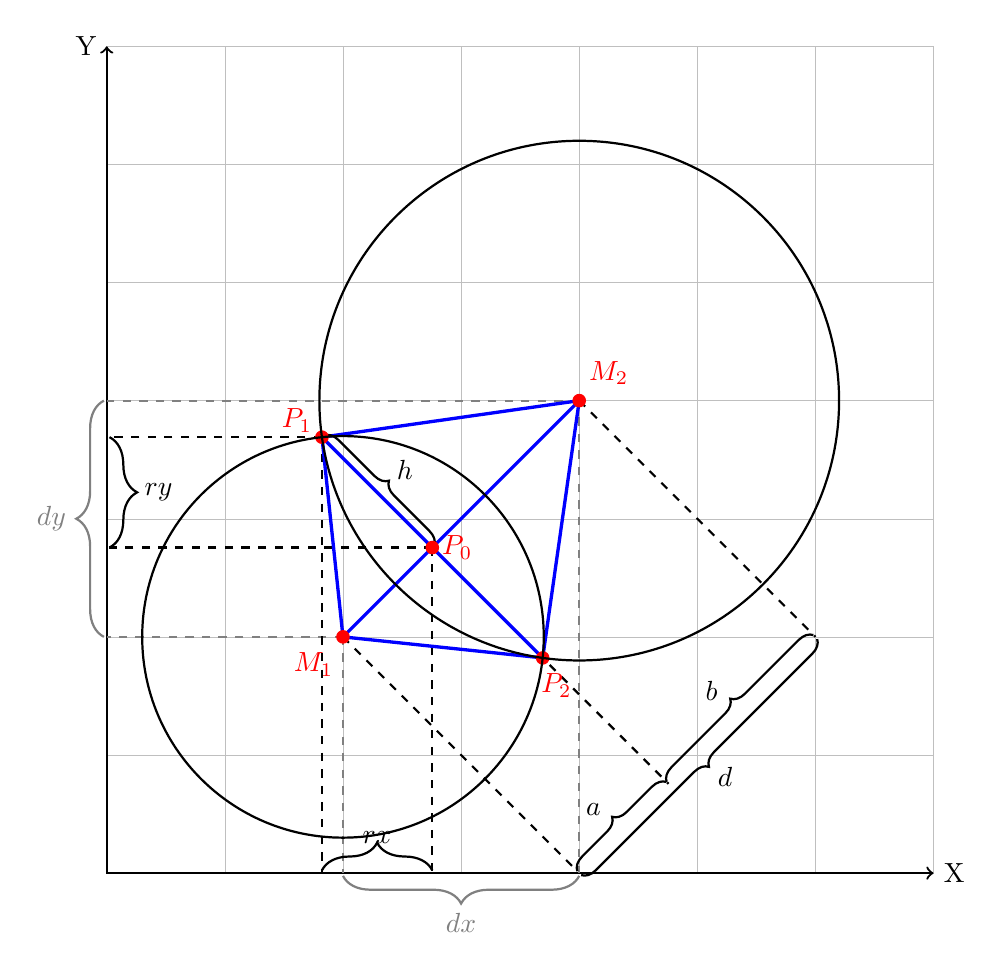
\begin{tikzpicture}[scale=1.5]
      
      % grid
      \draw[very thin,color=lightgray] (0,0) grid (7,7);
      \draw [<->,thick] (0,7) node (yaxis) [left] {Y} |- (7,0) node (xaxis) [right] {X};

      % radius of the circles
      \pgfmathsetlengthmacro{\radiusA}{1.7cm}
      \pgfmathsetlengthmacro{\radiusB}{2.2cm}
      
      % positions of circles and points
      \coordinate (A) at (2, 2);
      \coordinate (AX) at (2, 0);
      \coordinate (AY) at (0, 2);
      \coordinate (AZ) at (4, 0);
      \coordinate (B) at (4, 4);
      \coordinate (BX) at (4, 0);
      \coordinate (BY) at (0, 4);
      \coordinate (BZ) at (6, 2);
      \coordinate (C) at (2.75625, 2.75625);
      \coordinate (CX) at (2.75625, 0);
      \coordinate (CY) at (0, 2.75625);
      \coordinate (CZ) at (4.75625, 0.75625);
      \coordinate (D) at (1.8218593228739925,3.690640677126009);
      \coordinate (DX) at (1.8218593228739925,0);
      \coordinate (DY) at (0,3.690640677126009);
      \coordinate (E) at (3.690640677126009, 1.8218593228739917);
      
      % connect the positions
      \draw[thick,dashed,color=gray] (A) -- (AX);
      \draw[thick,dashed,color=gray] (A) -- (AY);
      \draw[thick,dashed] (A) -- (AZ);
      \draw[thick,dashed,color=gray] (B) -- (BX);
      \draw[thick,dashed,color=gray] (B) -- (BY);
      \draw[thick,dashed] (B) -- (BZ);
      \draw[thick,dashed] (C) -- (CX);
      \draw[thick,dashed] (C) -- (CY);
      \draw[thick,dashed] (C) -- (CZ);
      \draw[thick,dashed] (D) -- (DX);
      \draw[thick,dashed] (D) -- (DY);
      \draw[very thick,color=blue] (A) -- (B);
      \draw[very thick,color=blue] (A) -- (D);
      \draw[very thick,color=blue] (A) -- (E);
      \draw[very thick,color=blue] (B) -- (D);
      \draw[very thick,color=blue] (B) -- (E);
      \draw[very thick,color=blue] (D) -- (E);
      
      % curly braces
      \draw[thick,color=gray,decorate,decoration={brace,amplitude=10pt,mirror,raise=1pt}] (AX) -- (BX) node[midway,yshift=-18pt] {$dx$};
      \draw[thick,color=gray,decorate,decoration={brace,amplitude=10pt,raise=1pt}] (AY) -- (BY) node[midway,xshift=-20pt] {$dy$};
      \draw[thick,decorate,decoration={brace,amplitude=10pt,mirror,raise=1pt}] (CX) -- (DX) node[midway,above,yshift=7pt] {$rx$};
      \draw[thick,decorate,decoration={brace,amplitude=10pt,mirror,raise=1pt}] (CY) -- (DY) node[midway,right,xshift=10pt] {$ry$};
      \draw[thick,decorate,decoration={brace,amplitude=5pt,mirror,raise=1pt}] (AZ) -- (BZ) node[midway,xshift=10pt,yshift=-8pt] {$d$};
      \draw[thick,decorate,decoration={brace,amplitude=5pt,raise=1pt}] (AZ) -- (CZ) node[midway,xshift=-11pt,yshift=7pt] {$a$};
      \draw[thick,decorate,decoration={brace,amplitude=5pt,raise=1pt}] (CZ) -- (BZ) node[midway,xshift=-11pt,yshift=7pt] {$b$};
      \draw[thick,decorate,decoration={brace,amplitude=5pt,mirror,raise=1pt}] (C) -- (D) node[midway,xshift=10pt,yshift=8pt] {$h$};
      
      % mark the positions
      \draw[fill,color=red] (A) circle (1.5pt) node[left, yshift=-10pt] {$M_1$};
      \draw[fill,color=red] (B) circle (1.5pt) node[right, yshift=10pt] {$M_2$};
      \draw[fill,color=red] (C) circle (1.5pt) node[right] {$P_0$};
      \draw[fill,color=red] (D) circle (1.5pt) node[left, yshift=6pt] {$P_1$};
      \draw[fill,color=red] (E) circle (1.5pt) node[right, yshift=-10pt, xshift=-4pt] {$P_2$};
      
      % draw the circles
      \draw[thick,color=black] (A) circle (\radiusA);
      \draw[thick,color=black] (B) circle (\radiusB);
    \end{tikzpicture}
  % }
  \caption{Illustratie bij de methode voor het vinden van snijpunten tussen twee cirkels}
  \label{fig:snijpunten}
\end{figure}


\begin{figure}[!b]
  \centering
  \resizebox {\textwidth} {!} {
    \begin{tikzpicture}[scale=1.5]
      % grid
      \draw[very thin,color=lightgray] (0,0) grid (7,7);
      \draw [<->,thick] (0,7) node (yaxis) [left] {Y} |- (7,0) node (xaxis) [right] {X};
      
      
      \circle[1,2,1.5,1]
      \circle[2,4.5,2,1]    
      \circle[3,5.5,3,1]
      \circle[4,5,5.5,1]

      
    \end{tikzpicture}
  }
  \label{fig:voorbeeld_opgave}
  \caption{Het voorbeeld uit de opgave}
\end{figure}



\begin{figure}[H]
  \centering
  \resizebox {\textwidth} {!} {
    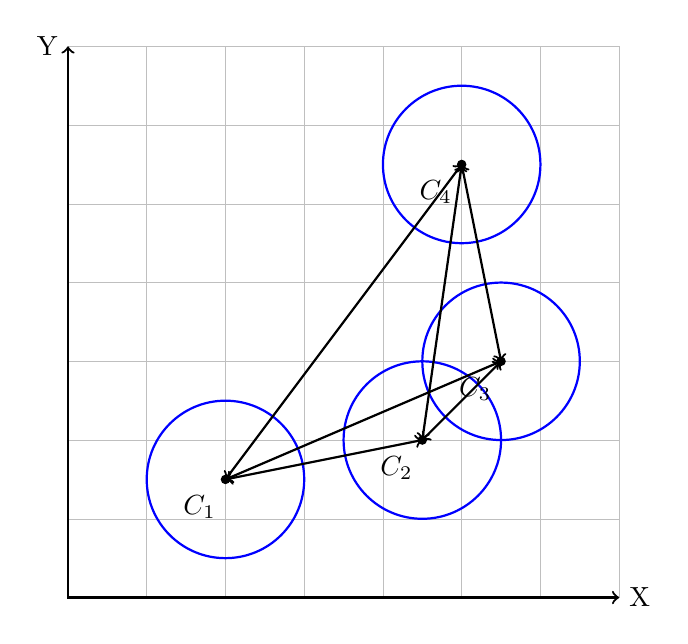
\begin{tikzpicture}[scale=1]
      % grid
      \draw[very thin,color=lightgray] (0,0) grid (7,7);
      \draw [<->,thick] (0,7) node (yaxis) [left] {Y} |- (7,0) node (xaxis) [right] {X};
      
      % Index, x, y, r
      \def\circle[#1,#2,#3,#4] {
    	% The middlepoint
    	\coordinate (C#1) at (#2,#3);
    	
    	% The point
        \draw[fill,color=black] (C#1) circle (1.5pt) node[left, yshift=-10pt, color=black] {$C_#1$};
        
        % The circle
        \draw[thick,color=blue] (C#1) circle (#4);

      }
      
      \circle[1,2,1.5,1]
      \circle[2,4.5,2,1]    
      \circle[3,5.5,3,1]
      \circle[4,5,5.5,1]
      

      \draw[thick,<->] (C1) -- (C2);
      \draw[thick,<->] (C1) -- (C3);
      \draw[thick,<->] (C1) -- (C4);
      \draw[thick,<->] (C2) -- (C3);
      \draw[thick,<->] (C2) -- (C4);
      \draw[thick,<->] (C3) -- (C4);

      
    \end{tikzpicture}
  }
  \label{fig:voorbeeld_1}
  \caption{Nagekeken cirkels bij algoritme 1}
\end{figure}
\begin{figure}[!b]
  \centering
  \resizebox {\textwidth} {!} {
    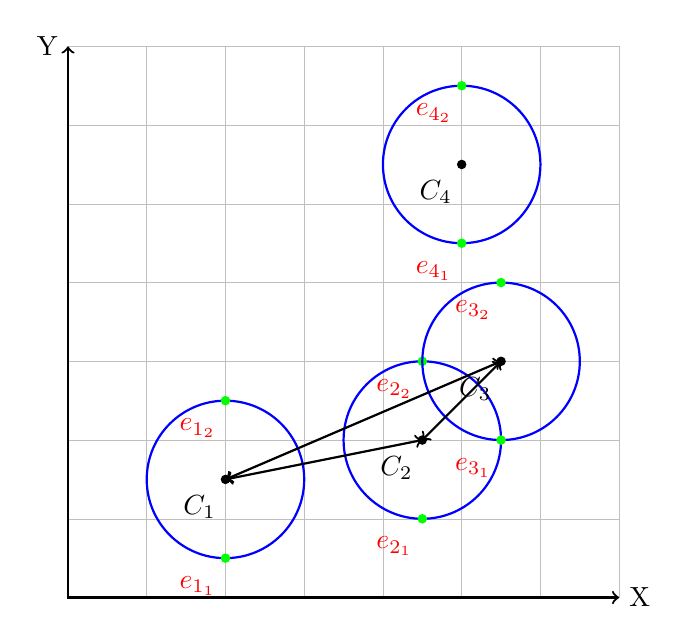
\begin{tikzpicture}[scale=1]
      % grid
      \draw[very thin,color=lightgray] (0,0) grid (7,7);
      \draw [<->,thick] (0,7) node (yaxis) [left] {Y} |- (7,0) node (xaxis) [right] {X};
      
      % Index, x, y, r
      \def\circle[#1,#2,#3,#4] {
    	% The middlepoint
    	\coordinate (C#1) at (#2,#3);
    	
    	
    	% The point
        \draw[fill,color=black] (C#1) circle (1.5pt) node[left, yshift=-10pt, color=black] {$C_#1$};
        
        % The circle
        \draw[thick,color=blue] (C#1) circle (#4);		
        
        % The eventpoints
        \coordinate (E#1_1) at (#2,#3-#4);
        \coordinate (E#1_2) at (#2,#3+#4);
    	
        \draw[fill, color=green] (E#1_1) circle (1.5pt) node[left, yshift=-10pt, color=red] {$e_{#1_1}$};
        \draw[fill, color=green] (E#1_2) circle (1.5pt) node[left, yshift=-10pt, color=red] {$e_{#1_2}$};
      }
      
      \circle[1,2,1.5,1]
      \circle[2,4.5,2,1]    
      \circle[3,5.5,3,1]
      \circle[4,5,5.5,1]
      

      \draw[thick,<->] (C1) -- (C2);
      \draw[thick,<->] (C1) -- (C3);
      \draw[thick,<->] (C2) -- (C3);


      
    \end{tikzpicture}
  }
  \label{fig:voorbeeld_2}
  \caption{Nagekeken cirkels bij algoritme 2}
\end{figure}
\begin{figure}[H]
  \centering
  % \resizebox {\textwidth} {!} {
    \begin{tikzpicture}[scale=1]
      % grid
      \draw[very thin,color=lightgray] (0,0) grid (7,7);
      \draw [<->,thick] (0,7) node (yaxis) [left] {Y} |- (7,0) node (xaxis) [right] {X};
      
      \indexedcircle[1,2,1.5,1]
      \indexedcircle[2,4.5,2,1]    
      \indexedcircle[3,5.5,3,1]
      \indexedcircle[4,5,5.5,1]

      \draw[thick,color=blue,arrows={Triangle[scale=1]-Triangle[scale=1]}] (C2) -- (C3);


      
    \end{tikzpicture}
  % }
  \label{fig:voorbeeld_23}
  \caption{Nagekeken cirkels bij algoritme 3}
\end{figure}

\begin{figure}[H]
  \centering
  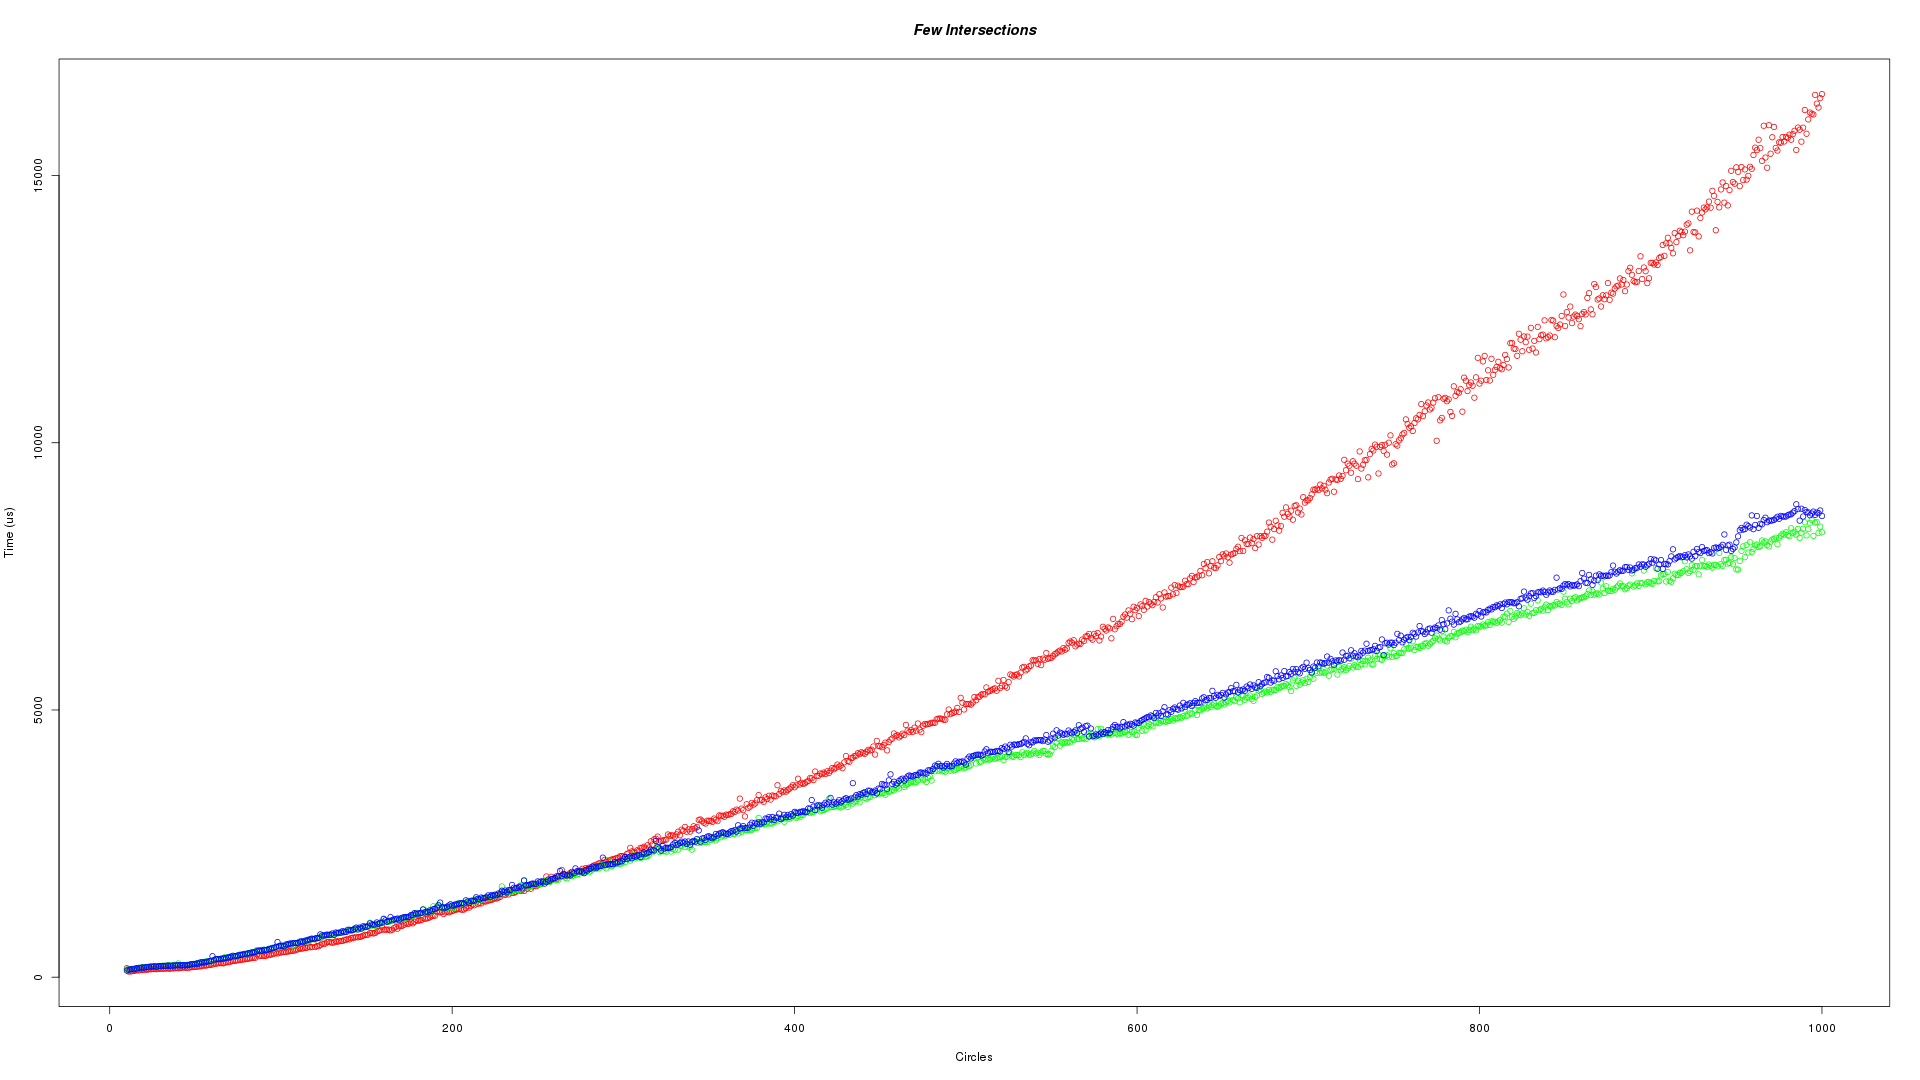
\includegraphics[width=1\textwidth]{illustraties/fewIntersections.png}
\end{figure}
\begin{figure}[H]
  \centering
  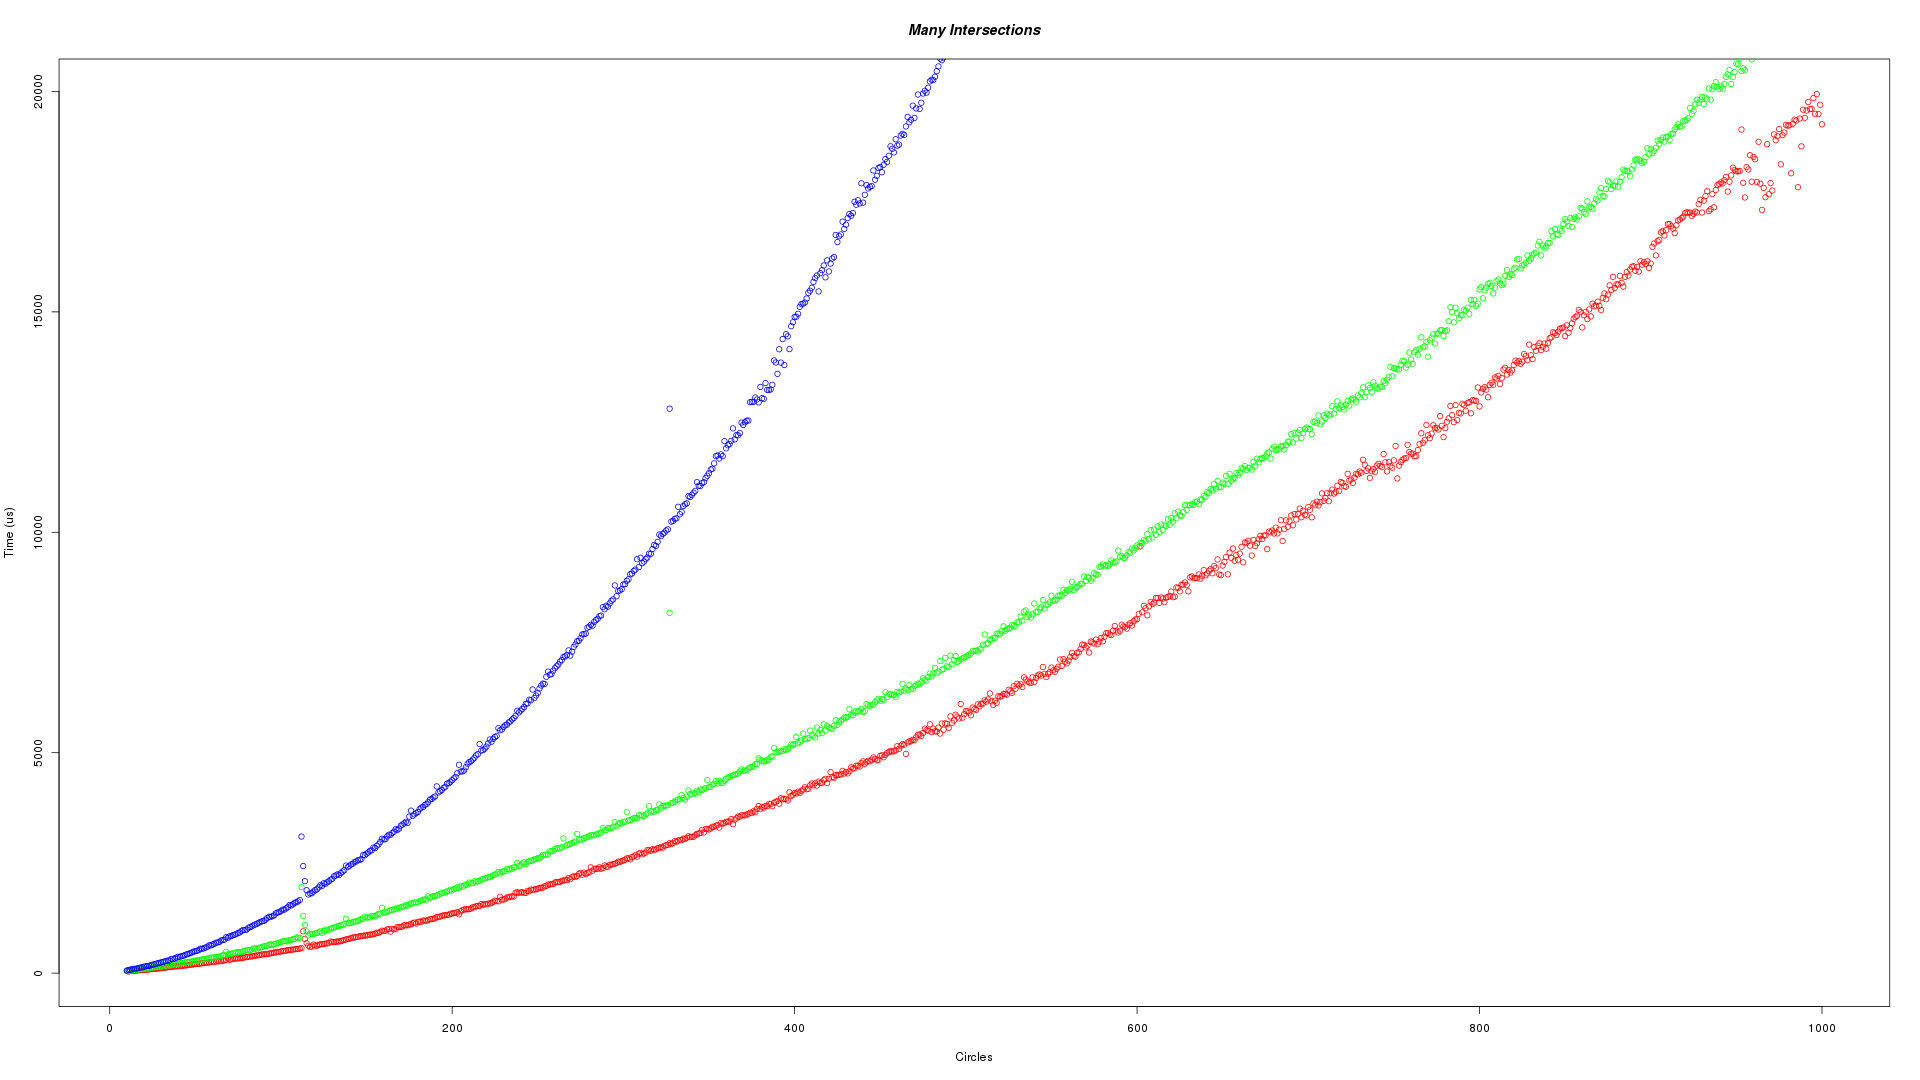
\includegraphics[width=1\textwidth]{illustraties/manyIntersections.png}
\end{figure}
\begin{figure}[H]
  \centering
  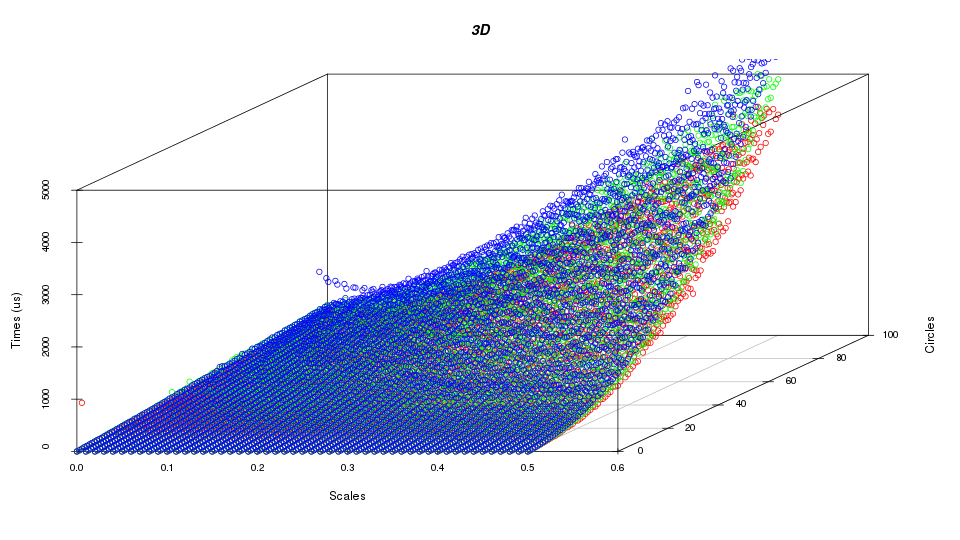
\includegraphics[width=1\textwidth]{illustraties/3DScatter.png}
\end{figure}



\section{Resultaten}
%% \todo{grafieken}

\section{Besluit}
%% \todo{besluit}

\listoftodos

\end{document}
